\setcounter{section}{25}

\section{Lecture 26: March 31}


\subsection*{Last time}
\begin{itemize}
	\item One-way ANOVA
\end{itemize}


\subsection*{Today}
\begin{itemize}
	\item Announcement: alternative grading path didn't pass (5:5 from last poll + a fail on the first poll)
	\item Analysis of Variance (JF chapter 8)
	  \begin{itemize}
	  	\item two-way ANOVA
	  \end{itemize}
\end{itemize}

\subsection*{Additional reference}
\href{https://www4.stat.ncsu.edu/~osborne/st512r/handouts/allpackets.pdf}{Course notes} by Dr. Jason Osborne.

\subsection*{Two-Way ANOVA}
The inclusion of a second factor permits us to model and test partial relationships, as well as to introduce interactions.
Let's take a look at the patterns of relationship that can occur when a quantitative response variable is classified by two factors.

\subsubsection*{Patterns of Means in the two-way classification}
Consider the following table:
	\begin{table}[H]
	\renewcommand{\arraystretch}{1.5}
	\centering
	\begin{tabular}{l|cccc|c}
		\toprule
		 & $C_1$ & $C_2$ & $\dots$ &$C_c$ & \\
		\hline
		$R_1$ & $\mu_{11}$ & $\mu_{12}$ & $\dots$ & $\mu_{1c}$  & $\mu_{1\cdot}$\\
		$R_2$ & $\mu_{21}$ & $\mu_{22}$ & $\dots$ & $\mu_{2c}$  & $\mu_{2\cdot}$\\
		$\vdots$ & $\vdots$ & $\vdots$ &  & $\vdots$  & $\vdots$\\
		$R_r$ & $\mu_{r1}$ & $\mu_{r2}$ & $\dots$ & $\mu_{rc}$  & $\mu_{r\cdot}$\\				
		\hline
		 & $\mu_{\cdot 1}$ & $\mu_{\cdot 2}$ & $\dots$ & $\mu_{\cdot c}$  & $\mu_{\cdot \cdot}$\\				
		\bottomrule
	\end{tabular}
\end{table}
The factors, $R$ and $C$ (for ``rows'' and ``columns'' of the table of means), have $r$ and $c$ categories, respectively.
The factor categories are denoted $R_j$ and $C_k$.
Within each cell of the design - that is, for each combination of categories $\{R_j, C_k\}$ of the two factors - there is a population cell mean $\mu_{jk}$ for the response variable.
Extending the dot notation, we have
$$
\mu_{j\cdot} \equiv \frac{\sum_{k = 1}^{c} \mu_{jk}}{c}
$$
is the \underline{marginal mean} of the response variable in row $j$.
$$
\mu_{\cdot k} \equiv \frac{\sum_{j = 1}^{r} \mu_{jk}}{r}
$$
is the marginal mean in column $k$. And
$$
\mu_{\cdot \cdot} \equiv \frac{\sum_j \sum_k \mu_{jk}}{r \times c}
$$
is the grand mean.

%
\begin{figure}[H]
	\begin{center}
		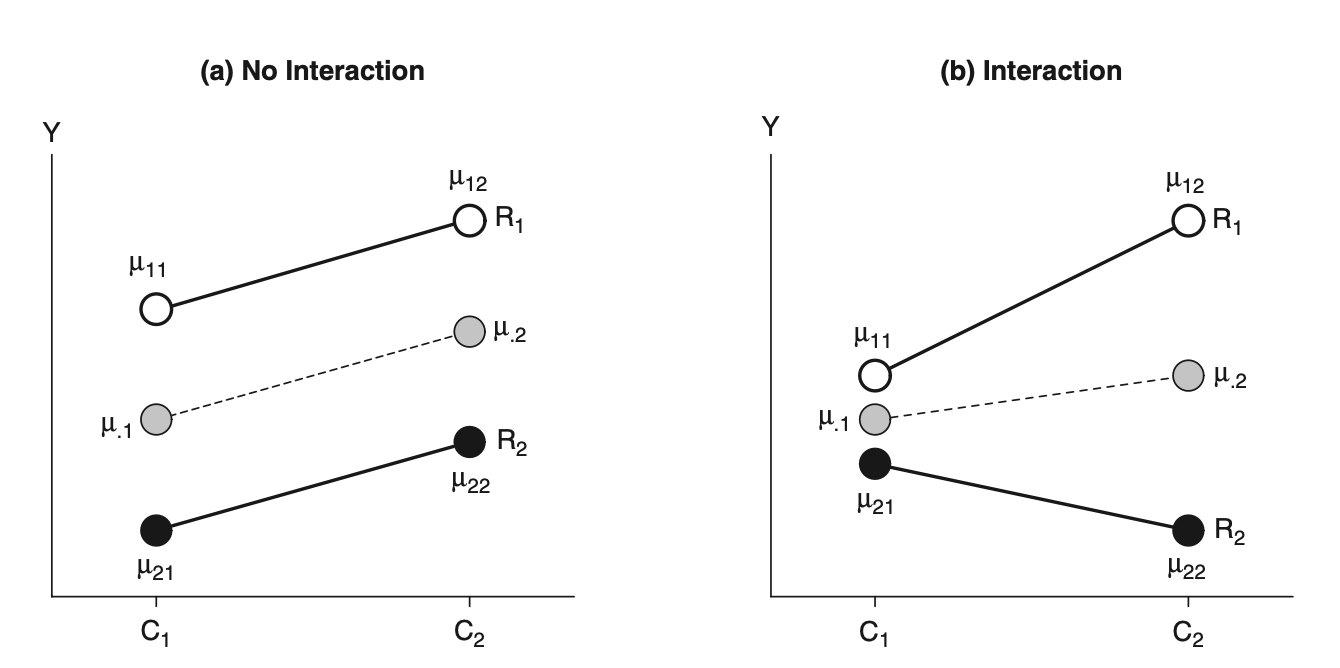
\includegraphics[width=0.9\textwidth]{Lecture25/JF_8_2}
		\caption{
			Interaction in the two-way classification.  In (a), the parallel profiles of means (given by the white and black circles connected by solid lines) indicate that $R$ and $C$ do not interact in affecting $Y$.
			The $R$-effect -- that is, the difference between the two profiles -- is the same at both $C_1$ and $C_2$.
			Likewise, the $C$-effect -- that is , the rise in the line from $C_1$ to $C_2$ -- is the same for both profiles.
			In (b), the $R$-effect differs at the two categories of $C$, and the $C$-effect differs at the two categories of $R$: $R$ and $C$ interact in affecting $Y$.
			In both graphs, the column marginal means $\mu_{\cdot 1}$ and $\mu_{\cdot 2}$ are shown as averages of the cell means in each column (represented by the gray circles connected by broken lines).
			JF Figure 8.2.}
		\label{fig:JF_8_2}
	\end{center}
\end{figure}
%
\subsubsection*{Two-way ANOVA model}
The two-way ANOVA model, suitably defined, provides a convenient means for testing the hypotheses concerning interactions and main effects.
The model is
$$
Y_{ijk} = \mu + \alpha_j + \beta_k + \gamma_{jk} + \epsilon_{ijk}
$$
where $Y_{ijk}$ is the $i$th observation in row $j$, column $k$ of the $RC$ table; $\mu$ is the general mean of $Y$; $\alpha_j$ and $\beta_k$ are the \underline{main-effect} parameters; $\gamma_{jk}$ are \underline{interaction effect} parameters; and $\epsilon_{ijk}$ are errors satisfying the usual linear-model assumptions (i.e.~$\epsilon_{ijk} \distas{iid} \mathcal{N}(0, \sigma^2)$).
By taking expectations, we have
$$
\mu_{jk} \equiv \textit{E}(Y_{ijk}) = \mu + \alpha_j + \beta_k + \gamma_{jk}
$$
We have $r \times c$ population cell means with $1 + r + c + r \times c$ model parameters.
Similar to one-way ANOVA model, we add in additional constraints to make the model identifiable.
$$
\begin{aligned}
	\sum\limits_{j = 1}^ r \alpha_j &= 0\\
	\sum\limits_{k = 1}^c \beta_k &= 0\\
	\sum\limits_{j = 1}^ r \gamma_{jk} &= 0 \quad \mbox{for all } k = 1, \dots, c\\
	\sum\limits_{k = 1}^c \gamma_{jk} &= 0 \quad \mbox{for all } j = 1, \dots, r\\
\end{aligned}
$$
The constraints produce the following solution for model parameters in terms of population cell and marginal means (and we add a hat for their estimates using the sample means):
$$
\begin{aligned}
	\mu &= \mu_{\cdot \cdot}\\
	\alpha_j &= \mu_{j \cdot} - \mu_{\cdot \cdot}\\
	\beta_k &= \mu_{\cdot k} - \mu_{\cdot \cdot} \\
	\gamma_{jk} &= \mu_{jk} - \mu - \alpha_j  - \beta_k \\
	&= \mu_{jk} - \mu_{j\cdot} - \mu_{\cdot k} + \mu_{\cdot \cdot}\\
\end{aligned}
$$

\subsubsection*{Hypotheses with two-way ANOVA}
Some interesting hypotheses:
\begin{enumerate}
	\item Are the cell means all equal? (Equivalent to one-factor ANOVA's ``overall F-test'')\\
	$H_0: \mu_{11} = \mu_{12} = \dots = \mu_{rc}$ vs. $H_a: \mbox{At least two } \mu_{ij} \mbox{ differ}$
	\item Are the marginal means for row main effect equal?\\
	$H_0: \mu_{1\cdot} = \mu_{2\cdot} = \dots = \mu_{r\cdot}$ vs $H_a: \mbox{At least two } \mu_{j\cdot} \mbox{ differ}$\\
	which is equivalent as testing for no row main effects $H_0: \mbox{all } \alpha_j = 0$ (why?)\\
	\begin{pf}
		{\it Answer: }
		This is because $\alpha_j = \mu_{j \cdot} - \mu_{\cdot \cdot}$ such that all $\alpha_j = 0$ is the equivalent as all marginal means are equal $\mu_{1\cdot} = \mu_{2\cdot} = \dots = \mu_{r\cdot}$.
	\end{pf}
	\item Are the marginal means for column main effect equal?\\
	$H_0: \mu_{\cdot 1} = \mu_{\cdot 2} = \dots = \mu_{\cdot c}$ vs $H_a: \mbox{At least two } \mu_{\cdot k} \mbox{ differ}$\\	
	\item Do the factors interact? In other words, does effect of one factor depend on the other factor?
	$H_0: \mu_{ij} = \mu_{\cdot \cdot} + (\mu_{i \cdot} - \mu_{\cdot \cdot}) + (\mu_{\cdot j} - \mu_{\cdot \cdot})$ vs $H_a: \mbox{At least one } \mu_{ij} \neq \mu_{\cdot \cdot} + (\mu_{i \cdot} - \mu_{\cdot \cdot}) + (\mu_{\cdot j} - \mu_{\cdot \cdot})$\\
	The null hypothesis is also equivalent as $H_0: \mbox{all } \gamma_{jk} = 0$.
\end{enumerate}

\subsubsection*{Testing hypotheses in two-way ANOVA}
We follow the notations of JF for incremental sums of squares in ANOVA:
$$
\begin{aligned}
	\textbf{SS}(\gamma | \alpha, \beta) &= \textbf{SS}(\alpha, \beta, \gamma) - \textbf{SS}(\alpha, \beta)\\
	\textbf{SS}(\alpha |  \beta, \gamma) &= \textbf{SS}(\alpha, \beta, \gamma) - \textbf{SS}(\beta, \gamma)\\
	\textbf{SS}(\beta |  \alpha, \gamma) &= \textbf{SS}(\alpha, \beta, \gamma) - \textbf{SS}(\alpha, \gamma)\\
	\textbf{SS}(\alpha | \beta) &= \textbf{SS}(\alpha, \beta) - \textbf{SS}(\beta)\\
	\textbf{SS}(\beta |  \alpha) &=\textbf{SS}(\alpha, \beta) - \textbf{SS}(\alpha)\\
\end{aligned}
$$
where $\textbf{SS}(\alpha, \beta, \gamma)$ denotes the regression sum of squares for the full model which includes both sets of main effects and the interaction. $\textbf{SS}(\alpha, \beta)$ denotes the regression sum of squares for the no-interaction model and $\textbf{SS}(\alpha, \gamma)$ denotes the regression for the model that omits the column main-effect regressors.
Note that the last model violates the principle of marginality because it includes the interaction regressors but omits the column main effects.
However, it is useful for constructing the incremental sum of squares for testing the column main effects.

{\it Additional readings: } \href{http://www.utstat.utoronto.ca/reid/sta442f/2009/typeSS.pdf}{Notes on 3 types of Sum of Squares }by Dr. Nancy Reid.

We now have the two-way ANOVA table
\begin{table}[H]
	\renewcommand{\arraystretch}{1.5}
	\caption{Two-way ANOVA table}
	\label{tab:one_way_anova_table}
	\centering
	\begin{tabular}{lccc}
		\toprule
		Source & Sum of Squares & df &  $H_0$\\
		\hline
		R & $\textbf{SS}(\alpha |  \beta, \gamma)$ & $r - 1$ & all $\alpha_j = 0$\\
		& $\textbf{SS}(\alpha |  \beta)$ & $r - 1$ & all $\alpha_j = 0 \mbox{ } | \mbox{ all } \gamma_{jk} = 0$\\
		\hline
		C & $\textbf{SS}(\beta |  \alpha, \gamma)$ & $c - 1$ & all $\beta_k = 0$\\
		   & $\textbf{SS}(\beta |  \alpha)$ & $c - 1$ & all $\beta_k = 0 \mbox{ } | \mbox{ all } \gamma_{jk} = 0$\\	
		\hline
		RC & $\textbf{SS}(\gamma | \alpha, \beta)$ & (r -1)(c - 1) &  all $\beta_k = 0$\\
		\hline
		Residuals & $\textbf{TSS} - \textbf{SS}(\alpha, \beta, \gamma)$ & n - rc &\\
		\hline
		Total &\textbf{TSS}& n -1 &\\
		\bottomrule
	\end{tabular}
\end{table}
where the residual sum of squares
$$
RSS = \sum\limits_i\sum\limits_j\sum\limits_k(Y_{ijk} - \bar{Y}_{jk})^2
$$

When test for the hypothesis, use the corresponding SS and df together with the residual SS and df to construct the $F$-statistic.
$$
F = \frac{SS/df}{RSS / df_{residual}}
$$
There are two reasonable procedures for testing main-effect hypotheses in two-way ANOVA:
\begin{enumerate}
	\item Tests based on $\textbf{SS}(\alpha | \beta, \gamma)$ and  $\textbf{SS}(\beta | \alpha, \gamma)$  (``type III'' tests) employ models that violate the principle of marginality, but the tests are valid whether or not interactions are present.
	\item Tests based on $\textbf{SS}(\alpha | \beta)$ and $\textbf{SS}(\beta | \alpha)$ (``type II'' tests) conform to the principle of marginality but are valid only if interactions are absent, in which case they are maximally powerful.
\end{enumerate}

Some more jargon:
\begin{itemize}
	\item Experimental unit (EU): entity to which experimental treatment is assigned.\\
	For example, Assign fertilizer treatment to fields.  Fields = EU.
	\item Measurement unit (MU): entity that is measured.\\
	For example, Measure yields at several subplots within each field.  MU: subplot
	\item Treatment structure: describes how different experimental factors are combined to generate treatments.\\
	For example, Fertilizers: A, B, C; Irrigation: High, Low.
	\item Randomization structure: how treatments are assigned to EUs.
	\item Simplest treatment structure: single experimental factor with multiple levels.  Ex. Fertilizers A vs B vs C.
	\item Simplest randomization structure: Completely randomized design -- Experimental treatments assigned to EUs entirely at random.
\end{itemize}

\subsubsection*{Example: Honeybee data}
Entomologist records energy expended ($y$) by $N=27$ honeybees at $a=3$ temperature (A) levels ($20, 30, 40^{\circ}C$) consuming liquids with $b = 3$ levels of sucrose concentration ($B$) ($20\%, 40\%, 60\%$) in a balanced, completely randomized crossed $3 \times 3$ design. 
\begin{table}[H]
	\renewcommand{\arraystretch}{1.5}
	\centering
	\begin{tabular}{cc|ccc}
		\toprule
		Temp & Suc & \multicolumn{3}{c}{Sample}\\
		\hline
		20 & 20 & 3.1 & 3.7 & 4.7\\
		20 & 40 & 5.5 & 6.7 & 7.3\\
		20 & 60 & 7.9 & 9.2 & 9.3\\
		30 & 20 & 6 & 6.9 & 7.5\\
		30 & 40 & 11.5 & 12.9 & 13.4\\
		30 & 60 & 17.5 & 15.8 & 14.7\\
		40 & 20 & 7.7 & 8.3 & 9.5\\
		40 & 40 & 15.7 & 14.3 & 15.9\\
		40 & 60 & 19.1 & 18.0 & 19.9\\
		
		\bottomrule
	\end{tabular}
\end{table}

\begin{enumerate}
	\item What is the experimental unit?\\
	\begin{pf}
		EU = honeybee.
	\end{pf}
	\item What is the treatment structure?\\
	\begin{pf}
		Three levels of temperature (A) are combined with each of the three sucrose concentrations (B).
	\end{pf}
	\item Finish the table below
\begin{table}[H]
	\renewcommand{\arraystretch}{1.5}
	\centering
	\begin{tabular}{lc}
		\toprule
		Source & df\\
		\hline
		A & \\
		B & \\
		$A \times B$ & \\
		Residual & \\
		\hline
		Total &\\
		\bottomrule
	\end{tabular}
\end{table}
{\it Answer: }\\
\begin{pf}
\begin{table}[H]
	\renewcommand{\arraystretch}{1.5}
	\centering
	\begin{tabular}{lr}
		\toprule
		Source & df\\
		\hline
		A & 2\\
		B & 2\\
		$A \times B$ & 4\\
		Residual & 18\\
		\hline
		Total &26\\
		\bottomrule
	\end{tabular}
\end{table}		
\end{pf}
\item 
Consider the model
$$
Y_{ijk} = \mu + \alpha_i + \beta_j + (\alpha \beta)_{ij} + \epsilon_{ijk}
$$
where $i = 1, 2, \dots, a$, $j = 1, 2, \dots, b$ and $k=1, 2, \dots, n$ for a balanced design.\\
Deviation:
\begin{itemize}
	\item total: $y_{ijk} - \bar{y}_{+++}$
	\item due to level $i$ of factor A: $\bar{y}_{i++} - \bar{y}_{+++}$
	\item due to level $j$ of factor B: $\bar{y}_{+j+} - \bar{y}_{+++}$	
	\item due to levels $i$ of factor A and $j$ of factor B after subtracting main effects:
	$$
	\bar{y}_{ij+} - \bar{y}_{+++} - (\bar{y}_{i++} - \bar{y}_{+++}) - (\bar{y}_{+j+} - \bar{y}_{+++}) = \bar{y}_{ij+} - \bar{y}_{i++} - \bar{y}_{+j+} + \bar{y}_{+++}
	$$
\end{itemize}
Use the following equations to calculate the Sum of Squares and fill out the ANOVA table.
$$
\begin{aligned}
SS[Tot] &= \sum\limits_i \sum\limits_j \sum\limits_k (y_{ijk} - \bar{y}_{+++})^2\\
SS[A] &= \sum\limits_i \sum\limits_j \sum\limits_k (\bar{y}_{i++}- \bar{y}_{+++})^2\\
SS[B] &= \sum\limits_i \sum\limits_j \sum\limits_k (\bar{y}_{+j+}- \bar{y}_{+++})^2\\
SS[AB] &= \sum\limits_i \sum\limits_j \sum\limits_k (\bar{y}_{ij+} - \bar{y}_{i++} - \bar{y}_{+j+} + \bar{y}_{+++})^2\\
SS[E] &= \sum\limits_i \sum\limits_j \sum\limits_k (\bar{y}_{ijk}- \bar{y}_{ij+})^2\\
\end{aligned}
$$
where
$$
\begin{aligned}
	\bar{y}_{ij+} &= \frac{1}{n} \sum\limits_k y_{ijk}\\ 
	\bar{y}_{i++} &= \frac{1}{b} \sum\limits_j \bar{y}_{ij+} = \frac{1}{bn} \sum\limits_j \sum\limits_k y_{ijk}\\ 
	\bar{y}_{+j+} &= \frac{1}{a} \sum\limits_i \bar{y}_{ij+}= \frac{1}{an} \sum\limits_i \sum\limits_k y_{ijk}\\ 
	\bar{y}_{+++} &= \frac{1}{a} \sum\limits_i \bar{y}_{i++}= \frac{1}{b} \sum\limits_j \bar{y}_{+j+}\\
	&= \frac{1}{abn} \sum\limits_i \sum\limits_j \sum\limits_k y_{ijk}
\end{aligned}
$$

\begin{table}[H]
	\renewcommand{\arraystretch}{1.5}
	\centering
	\begin{tabular}{lrrrr}
		\toprule
		Source & df & Sum of Squares & Mean Square & F\\
		\hline
		A & & & &\\
		B & & & &\\
		$A \times B$ & & & &\\
		Residual & & & &\\
		\hline
		Total & & & &\\
		\bottomrule
	\end{tabular}
\end{table}
{\it Answer: }\\
\begin{pf}
\begin{table}[H]
	\renewcommand{\arraystretch}{1.5}
	\centering
	\begin{tabular}{lrrrr}
		\toprule
		Source & df & Sum of Squares & Mean Square & F\\
		\hline
		Temp & 2 & 293.16 & 146.58 & 162.00\\
		Suc & 2 & 309.96 & 154.98 &171.28\\
		Temp $\times$ Suc & 4 & 27.13 & 6.78 &7.50\\
		Residual & 18 & 16.29 & 0.90 &\\
		\hline
		Total & 26 & 646.53 & &\\
		\bottomrule
	\end{tabular}
\end{table}	
\end{pf}
\end{enumerate}
%http://www.sthda.com/english/wiki/two-way-anova-test-in-r


















